\documentclass[10pt,a4paper]{article}

%% packages
\usepackage{color}
\usepackage{pgf}
\usepackage[margin=1in]{geometry}
\usepackage[normalem]{ulem}
\usepackage{cite}
\usepackage{natbib}
\usepackage{authblk}
\usepackage{listings}
\usepackage{color}
\usepackage[colorlinks=true,
            linkcolor=red,
            urlcolor=blue,
            citecolor=gray]{hyperref}
 
\definecolor{dkgreen}{rgb}{0,0.6,0}
\definecolor{gray}{rgb}{0.5,0.5,0.5}
\definecolor{mauve}{rgb}{0.58,0,0.82}
           
\lstset{frame=tb,
  language=bash,
  frame=none,
  aboveskip=3mm,
  belowskip=3mm,
  showstringspaces=false,
  columns=flexible,
  basicstyle={\small\ttfamily},
  numbers=none,
  numberstyle=\tiny\color{gray},
  keywordstyle=\color{blue},
  commentstyle=\color{dkgreen},
  stringstyle=\color{mauve},
  breaklines=true,
  breakatwhitespace=true,
  tabsize=3
}

\usepackage[colorinlistoftodos]{todonotes}
\definecolor{flame}{rgb}{0.89, 0.35, 0.13}
%\setlength{\marginparwidth}{1.5cm}
\newcommand{\jri}[1]{\todo[size=\scriptsize, color=flame]{#1}}
\newcommand{\ad}[1]{\todo[size=\scriptsize, color=blue]{#1}}
\newcommand{\ph}[1]{\todo[size=\scriptsize, color=pink]{#1}}
\newcommand{\tjyk}[1]{\todo[size=\scriptsize, color=green]{#1}}
\newcommand{\fst}{${F_{ST}}$ }          
\newcommand{\X}{\textcolor{red}{\bf X }}


%\title{More than one Author with different Affiliations}
\author[1,$\dag$]{Arun Durvasula}
\author[2,$\dag$]{Paul J. Hoffman}
\author[1]{Tyler V. Kent}
\author[2]{Chaochih Liu}
\author[2]{Thomas J. Y. Kono}
\author[2]{Peter L. Morrell}
\author[1,3,*]{Jeffrey Ross-Ibarra}
\affil[1]{Department of Plant Sciences, University of California, Davis, CA 95616}
\affil[2]{Department of Agronomy and Plant Genetics, University of Minnesota, St. Paul, MN 55108}
\affil[3]{Center for Population Biology and Genome Center, University of California, Davis, CA 95616}
\affil[$\dag$]{These authors contributed equally.}
\affil[*]{email: rossibarra@ucdavis.edu}


\renewcommand\Authands{ and }

\begin{document}

\title{ANGSD-wrapper: utilities for analyzing next generation sequencing data}
\maketitle

\begin{abstract}
High throughput sequencing has changed many aspects of population genetics, molecular ecology, and related fields, affecting both experimental design and data analysis.
The software package ANGSD allows users to perform a number of population genetic analyses on high-throughput sequencing data. 
The package is specifically designed to produce more accurate results for samples with low sequencing depth and makes use of full genome data while handling a wide array of sampling and experimental designs.
Here we present ANGSD-wrapper, a user-friendly interface for running ANGSD and visualizing results.
ANGSD-wrapper includes a number of 'wrapper' scripts that facilitate configuration and execution of multi-step analyses. ANGSD-wrapper also provides interactive graphing of ANGSD results to enhance data exploration.
We demonstrate the usefulness of ANGSD-wrapper by analyzing resequencing data from populations of wild and domesticated \textit{Zea}. 
ANGSD-wrapper is freely available from \url{https://github.com/mojaveazure/angsd-wrapper}.
\end{abstract}

\section*{Introduction}

High throughput sequencing has revolutionized evolutionary genetics, allowing researchers to quickly assay large numbers of individuals or survey fine-scale patterns of variation across the genome. 
Application of these approaches has led to changes in both experimental design and data analysis \citep{ekblom2011applications}.
Many popular software packages used by researchers for analysis of comparative resequencing data \citep[see][]{excoffier2006computer} were not designed to handle these novel data types or efficiently analyze the large volumes of data now being generated. 
Despite the decreasing cost of sequencing, researchers must allocate finite resources and balance the depth of sequencing and the breadth of a sample. 
This poses a challenge for population genetics analysis, which generally requires accurate polymorphism calls in a broad sample. 
This is especially true of studies that span multiple subpopulations, as this balance must be met for each partition \citep{pluzhnikov1996optimal, felsenstein2006accuracy}. 
While the experimental design challenges with molecular population genetic studies have existed for at least a decade, high throughput sequencing brings the technical challenges of highly variable coverage, missing data, and high per-nucleotide error rates.

A number of tools have recently been published to estimate population genetic descriptive statistics using high throughput sequencing data \citep{garrigan2013popbam, purcell2007plink, danecek2011variant, hutter2006genome}. 
However, few of these tools offer the flexibility to handle data with low coverage and high missingness, resulting in either high data loss or bias in estimates. 
Korneliussen et al. \ph{Should be just \(2014\)} \citep{korneliussen2014angsd} recently published the software package, ANGSD, which enables users to flexibly perform a large number of common population genetic analyses, including estimation of diversity statistics, admixture analysis including Patterson's D statistic \citep{Durand:2011jd}, site frequency spectrum estimation \citep{pmid22911679}, and calculation of neutrality test statistics \citep{korneliussen_calculation_2013}. 
ANGSD works directly with the alignment formats produced from standard high throughput sequence analysis pipelines, which removes the need for the user to transform the data into a niche format. 
One of the most important features of ANGSD is that analyses are integrated over per-site genotype likelihoods, rather than only on pre-determined variable sites. 
This permits ANGSD to calculate common population genetic descriptive statistics on low-coverage sequencing data, and handle missingness due to variation in coverage. 

Here we present ANGSD-wrapper, a user-friendly interface to stable versions of ANGSD. 
ANGSD-wrapper takes the form of a set of configuration files and `wrapper' scripts (Figure \ref{fig:supp2}) that streamline the execution of multi-step pipelines required for data analysis in ANGSD. 
ANGSD-wrapper also eases the configuration of ANGSD-related programs such as \tjyk{Fumagali citation doesn't show up properly}ngsPopGen \citep{ngsPopGen}, ngsF\citep{vieira2013estimating}, and ngsAdmix \citep{pmid24026093}. 
Additionally, the wrapper scripts are written against ``frozen'' versions of ANGSD and supporting tools, for consistency of analysis. 
Because the large volume of data associated with high throughput sequence analysis is often difficult to visualize, ANGSD-wrapper also provides a suite of interactive visualization tools to plot results and explore patterns at multiple scales.  
We demonstrate some of the analyses possible using ANGSD-wrapper when applied to low-coverage whole-genome data from domesticated maize and two related wild teosinte subspecies. 
ANGSD-wrapper is freely available from \url{https://github.com/mojaveazure/angsd-wrapper}.

\section*{Methods}
\ph{change of language} ANGSD-wrapper is a set of configuration files and scripts written primarily in the Bash scripting language. %UNIX shell.  
The scripts can be run either on a standalone computer with a UNIX terminal, \ph{has anyone tested AW on a cluster?} or on computing clusters where they can be submitted to a queuing system such as SGE \citep{Microsystems):2001:SGE:560889.792378}, Slurm \citep{Jette02slurm:simple} or TORQUE \citep{Staples:2006:TRM:1188455.1188464}.  
A Python installation \citep{Python} is required for some light, dynamic pre-processing of the data.
An installation of the statistical software R \citep{Rcitation} is required to make use of the visualization tools incorporated in ANGSD-wrapper.  
The visualization portion of ANGSD-wrapper also requires installation of the R packages \texttt{Shiny} \citep{shiny}, \texttt{APE} \citep{APE}, \texttt{Lattice} \citep{lattice}, \texttt{Hmisc} \citep{Hmisc}, \texttt{data.table} \citep{datatable}, \texttt{DT} \citep{javascriptDT}, and \texttt{shinythemes} \citep{shinythemes}, as well as \texttt{genomeIntervals} \citep{genomeIntervals} from Bioconductor \citep{bioconductor} for the visualization package.
These dependent packages are installed automatically upon first run of visualization interface.


\begin{table}
\begin{center}
    \begin{tabular}{ | p{3.5cm} | p{5cm} | p{2.5cm}  |}
    \hline
    \textbf{Method} & \textbf{Calculations} & \textbf{Interactive Graphing} \\ \hline
    SFS     &    Site frequency spectrum  & Yes  \\ \hline     2DSFS   &    Joint site frequency spectrum, \fst & Yes  \\ \hline 
    ABBA/BABA  &  Patterson's D statistic & Yes  \\ \hline 
    Ancestral &  Extract ancestral sequence from BAM file  & No \\ \hline 
    Genotypes &  Genotype likelihood estimations & No  \\ \hline 
    PCA     &    Principal component analysis & Yes  \\ \hline 
    Thetas   &   Diversity statistics ($\theta_w$, $\theta_\pi$, Fu and Li's $\theta$, Fay's $\theta$) and neutrality tests (Tajima's D, Fu and Li's D, Fu and Li's F,  Fay and Wu's H, Zeng's E ) & Yes  \\ \hline 
    Inbreeding & Calculate per-individual inbreeding coefficients with ngsF & No  \\ \hline 
    Admixture  & Perform admixture analysis & Yes  \\ \hline 
    \end{tabular}
    \caption{Table of methods implemented in ANGSD-wrapper}
    \label{tab:methods}
    \end{center}
\end{table}

ANGSD-wrapper is divided into scripts associated with analytical approaches implemented in ANGSD and associated software. 
ANGSD-wrapper provides a common configuration file, \texttt{Common\_Config}, which holds variables that are likely to remain constant across analyses, including identifiers for chromosomal regions and the paths to project directories.
In ANGSD-wrapper, each method is self-contained in a shell script which uses information from the common configuration file and a method-specific configuration file. 
Each analysis is run using a simple command:

\begin{lstlisting}
$ angsd-wrapper <method> <configuration_file>
\end{lstlisting}

Analyses supported by ANGSD-wrapper are shown in Table \ref{tab:methods}.
A detailed flowchart of each of these workflows is shown in Figure \ref{fig:supp2}, and additional details, documentation, a tutorial, and a wiki can be found on the GitHub page: \url{https://github.com/mojaveazure/angsd-wrapper/wiki}.

The visualization software included with ANGSD-wrapper is contained within its own directory called ``shinyGraphing.''
This application is started from within ANGSD-wrapper and launched locally from a standard web browser. %This application must be started in R and can be accessed locally from a web browser. --Nope
This software provides a graphical user interface (GUI) to quickly and interactively plot results obtained from ANGSD-wrapper.  
Each tab in the GUI contains plots for different ANGSD methods.

In order to use the plotting software, the user navigates to the desired tab and uploads the appropriate results file. 
The Shiny server automatically parses ANGSD output files and creates the resulting plot(s) (Figure \ref{fig:theta}), which can be saved using the browser's built in image saving capabilities.

\begin{figure}
\centering
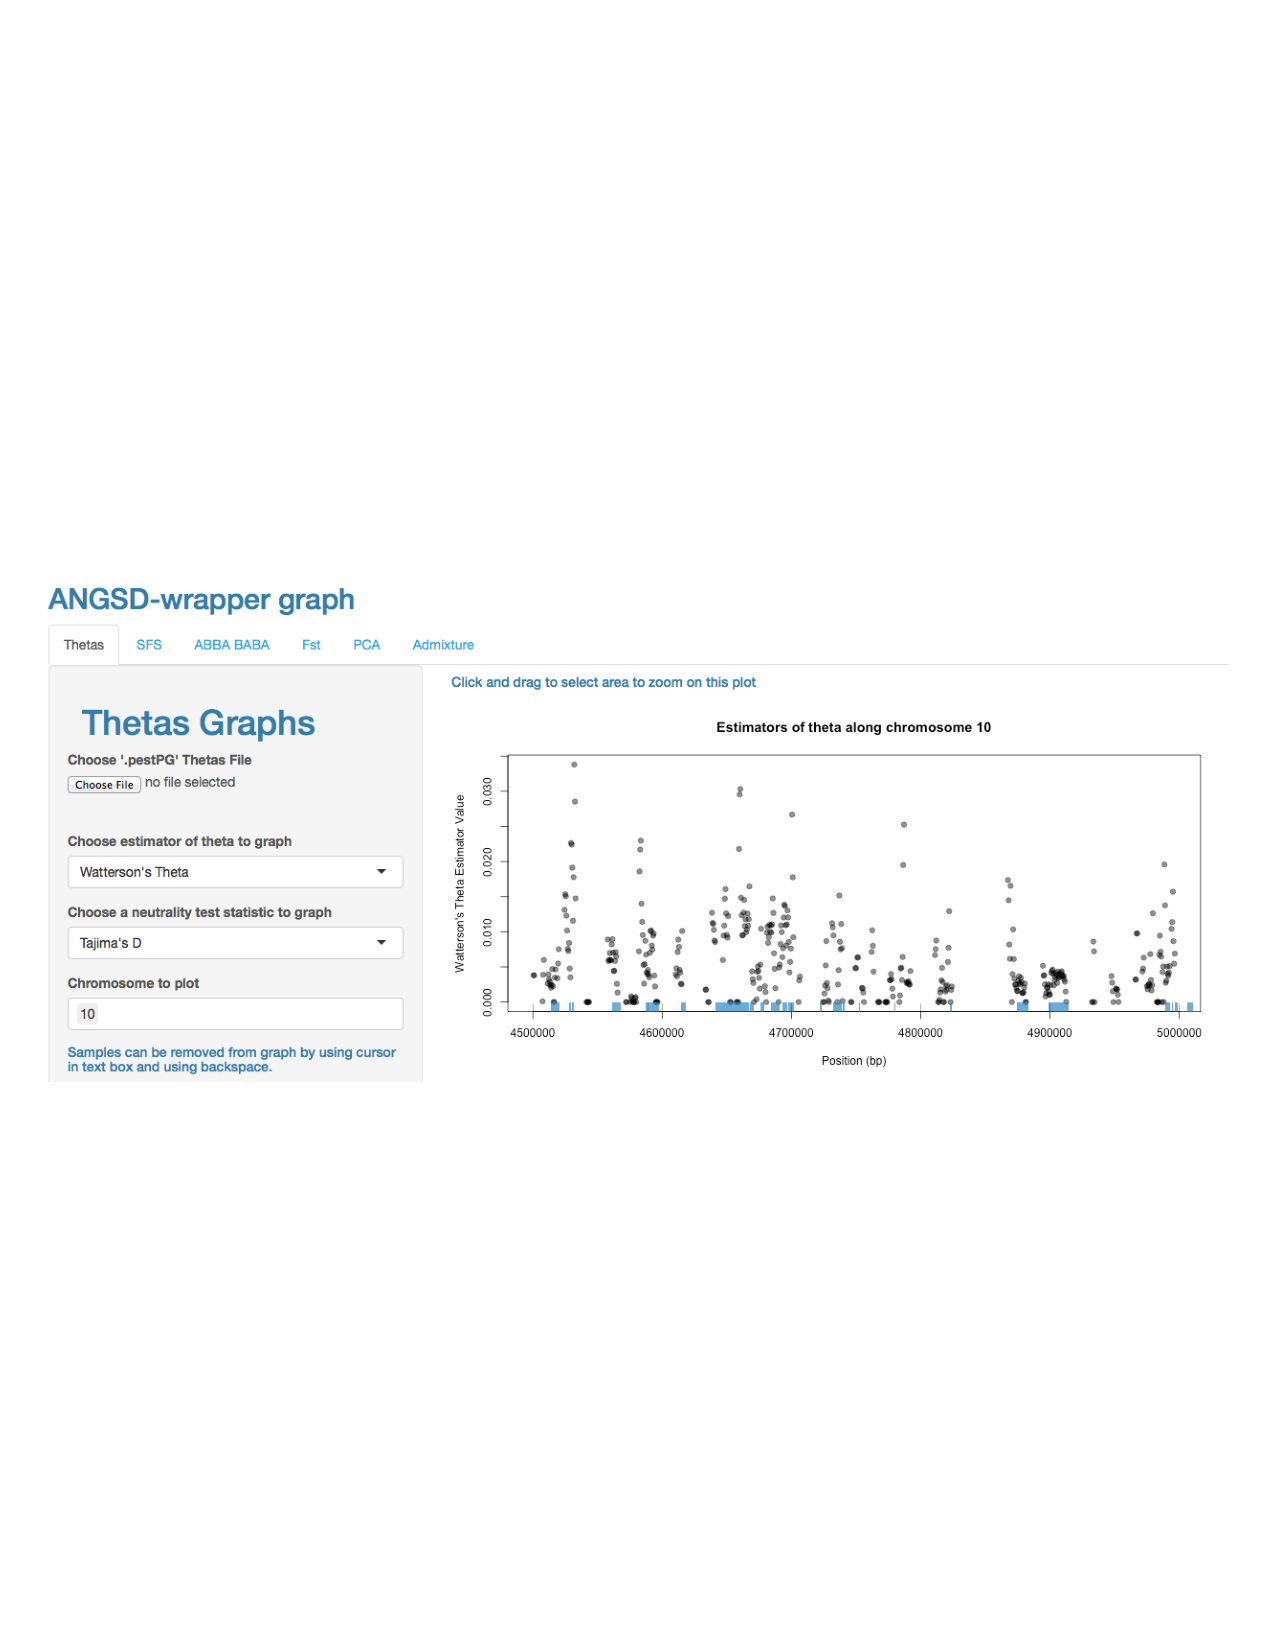
\includegraphics[width=0.8\linewidth]{figures/fig1.pdf}
\caption{Visualization of Watterson's $\theta$ estimated by ANGSD across a 1.5Mb region of chromosome 10 in {\it Zea mays} ssp. {\it mays} using ANGSD-wrapper. Darker colors indicate a higher density of points. Blue boxes indicate gene annotations provided by a GFF file. \label{fig:theta} }
\end{figure}

\begin{figure}
\centering
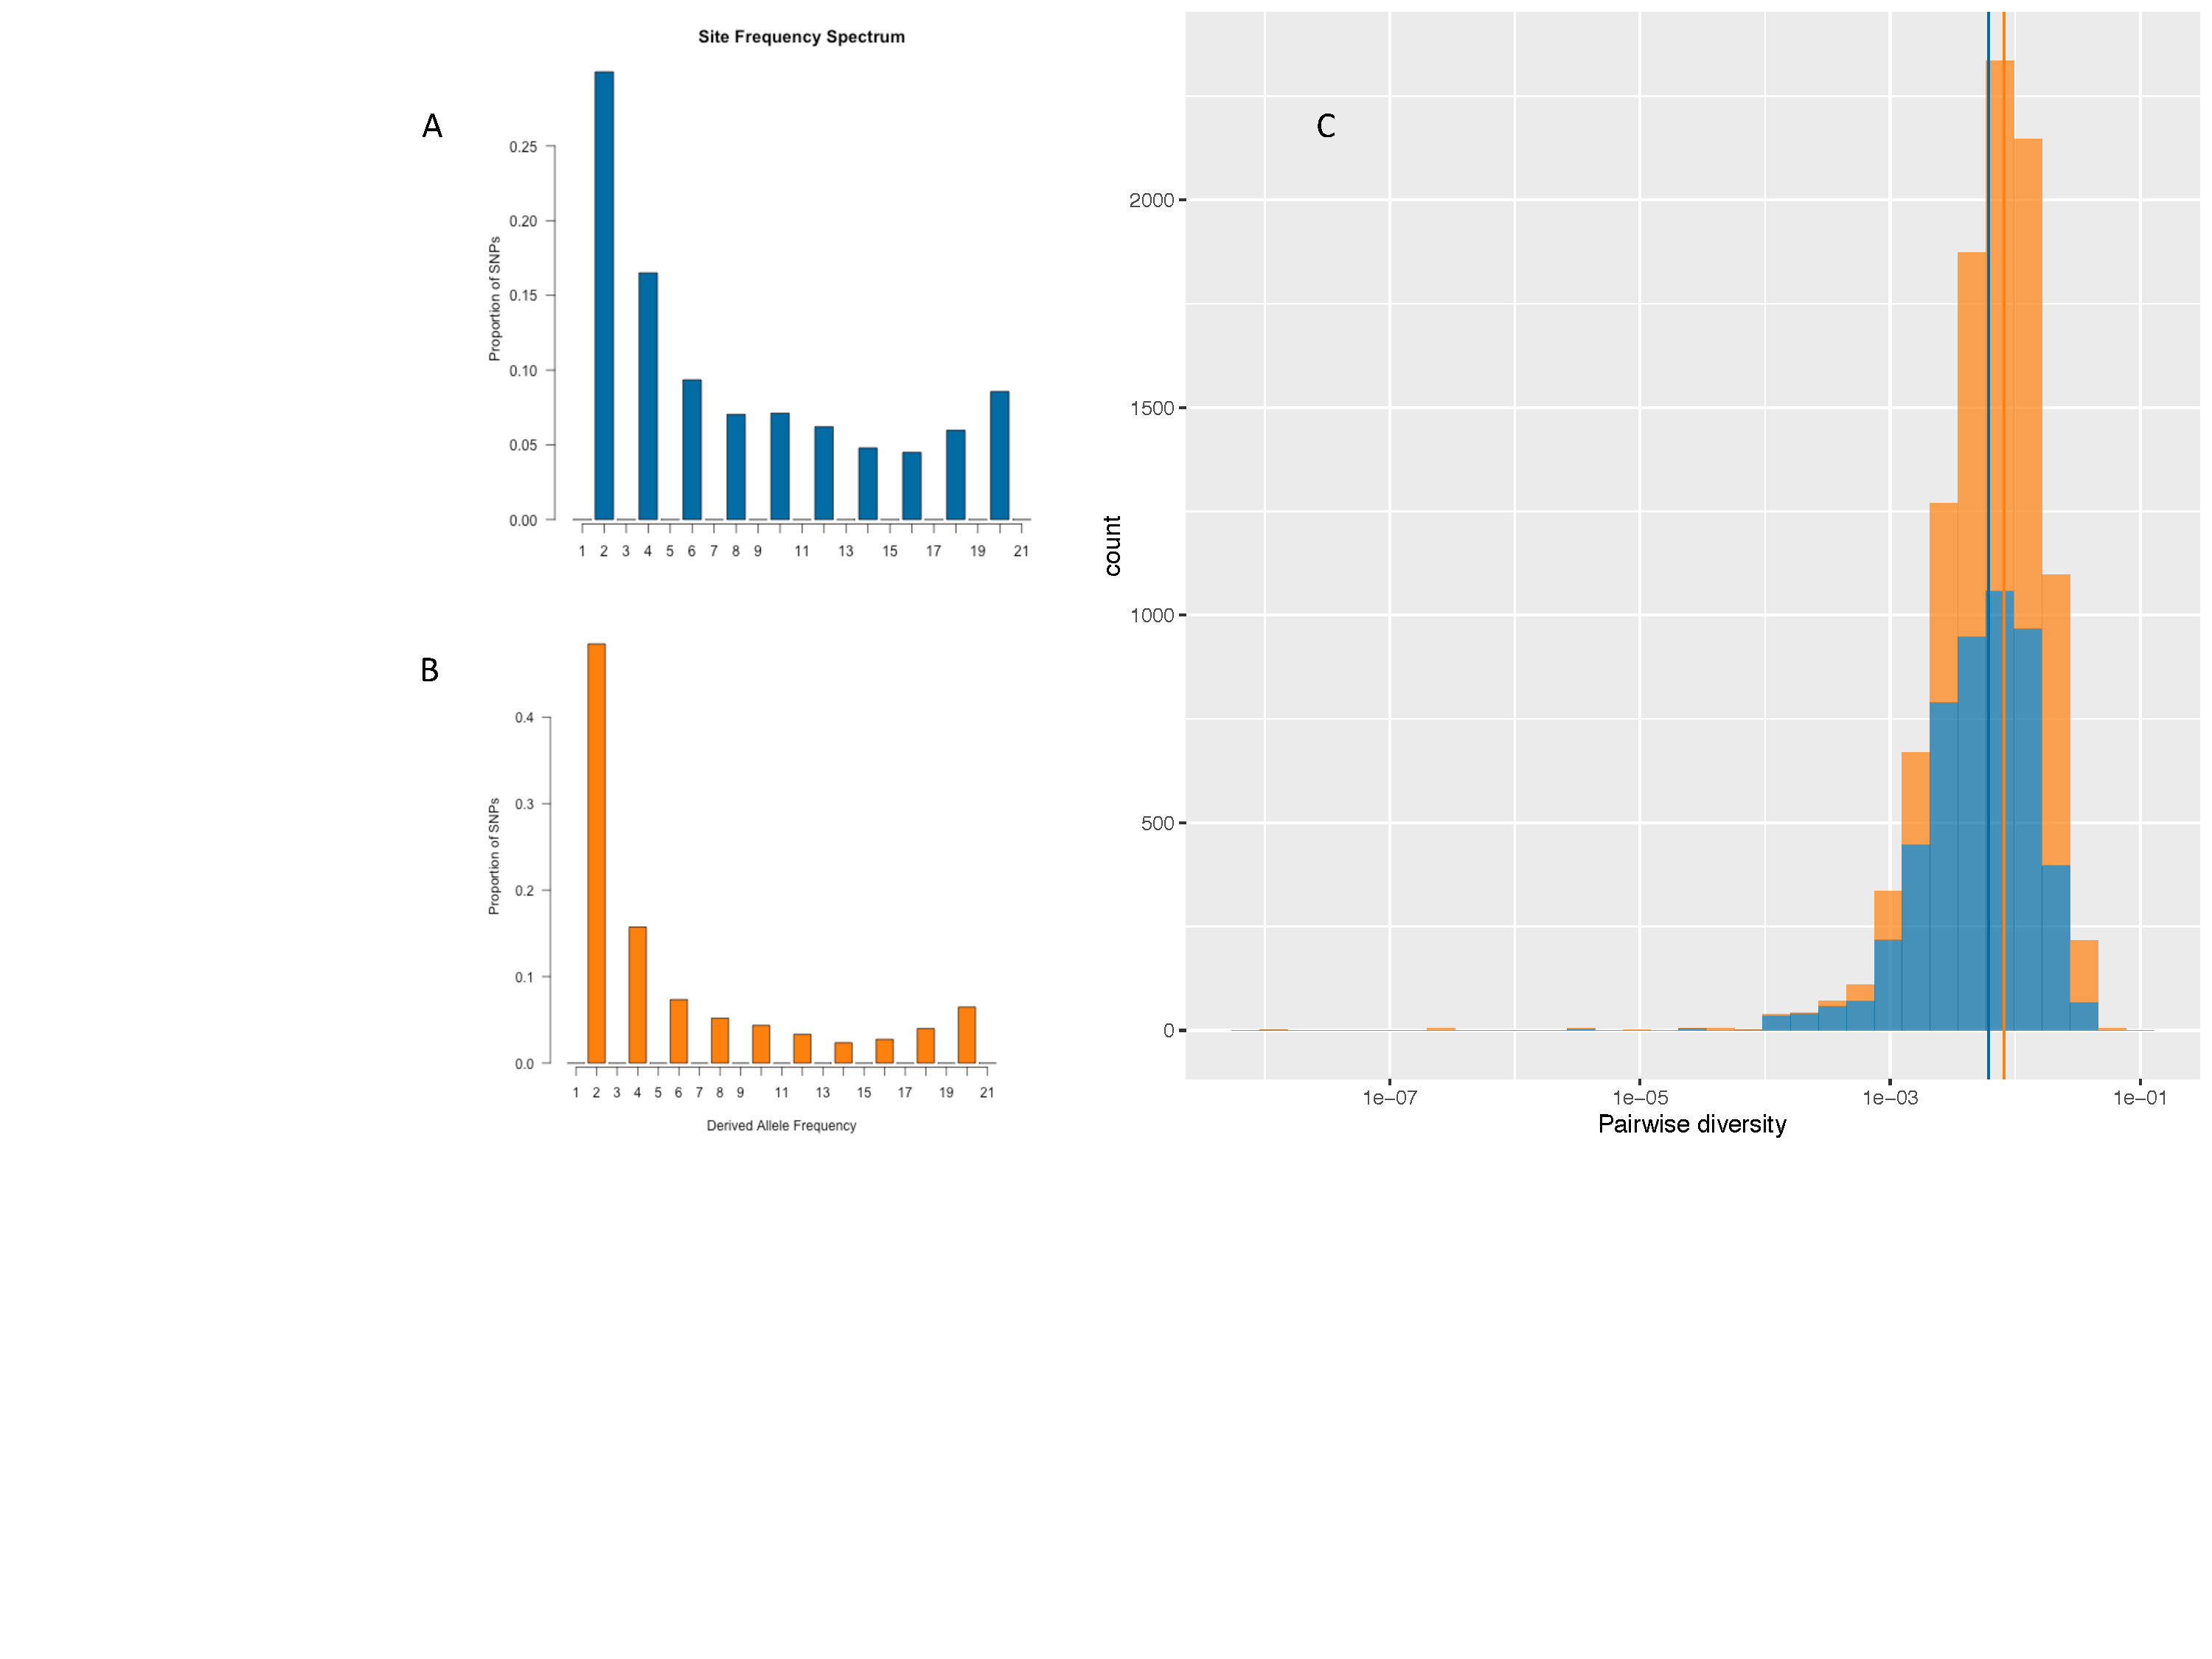
\includegraphics[width=0.8\linewidth]{figures/figure3big.pdf}
\caption{Summary statistics for {\it Zea mays}. Derived site frequency spectra for A. maize and B. teosinte. C. distribution of pairwise differences for maize (blue) and teosinte (orange). Pairwise diversity results are visualized separately from the interactive graphics and colors were added to A and B using a custom script.}
\label{fig:figure3}
\end{figure}
\tjyk{Should this start a "Results" section?}
As a demonstration of analyses in ANGSD-wrapper, we explore patterns of diversity in a single genomic region of domesticated maize and wild teosinte. 
We used a subset of the resequenced samples from the Maize HapMap2 project (Table \ref{tab:samples}) and calculated summary statistics using a 10Mb region on chromosome 10 \citep{chia2012maize}. 
The data are available at \url{https://figshare.com/articles/Example_Data_tar_bz2/2063442}. 
In the following we refer to methods listed in Table \ref{tab:methods} when describing analyses.

We first use the ``SFS'' method to estimate the site frequency spectrum (SFS) of both maize and its wild progenitor \textit{Zea mays} ssp. \textit{parviglumis}, assuming an inbreeding coefficient of $F=1$ for these highly inbred samples. 
The SFS and diversity statistics were calculated using ancestral states inferred in the ``Ancestral Sequence'' method from a single resequenced genome of \textit{Tripsacum dactyloides}.  
We show that the maize SFS is skewed towards more intermediate-frequency variants (Figure \ref{fig:figure3}A-B, Tajima's D of 0.2 and 0.0085 in maize and teosinte, respectively), likely a result of the bottleneck associated with maize domestication \citep{eyre1998investigation, Beissinger031666}.
Using the ``Thetas'' method we find further evidence of the domestication bottleneck, with mean levels of pairwise nucleotide diversity in this region in maize $\approx 25\%$ lower than in teosinte (0.0061 and 0.0082, respectively; Figure \ref{fig:figure3}C). 
Using the ``2DSFS method,'' which includes an \fst calculation, we find a mean \fst in this region of 0.116, nearly identical to the  genome-wide value of 0.11 reported in \cite{hufford2012comparative}.   
There are no genes in this region that have  been identified as potential domestication candidates, consistent with the lack of extended regions of high \fst in our analysis (Figure \ref{fig:suppfst}).

\begin{figure}
\centering
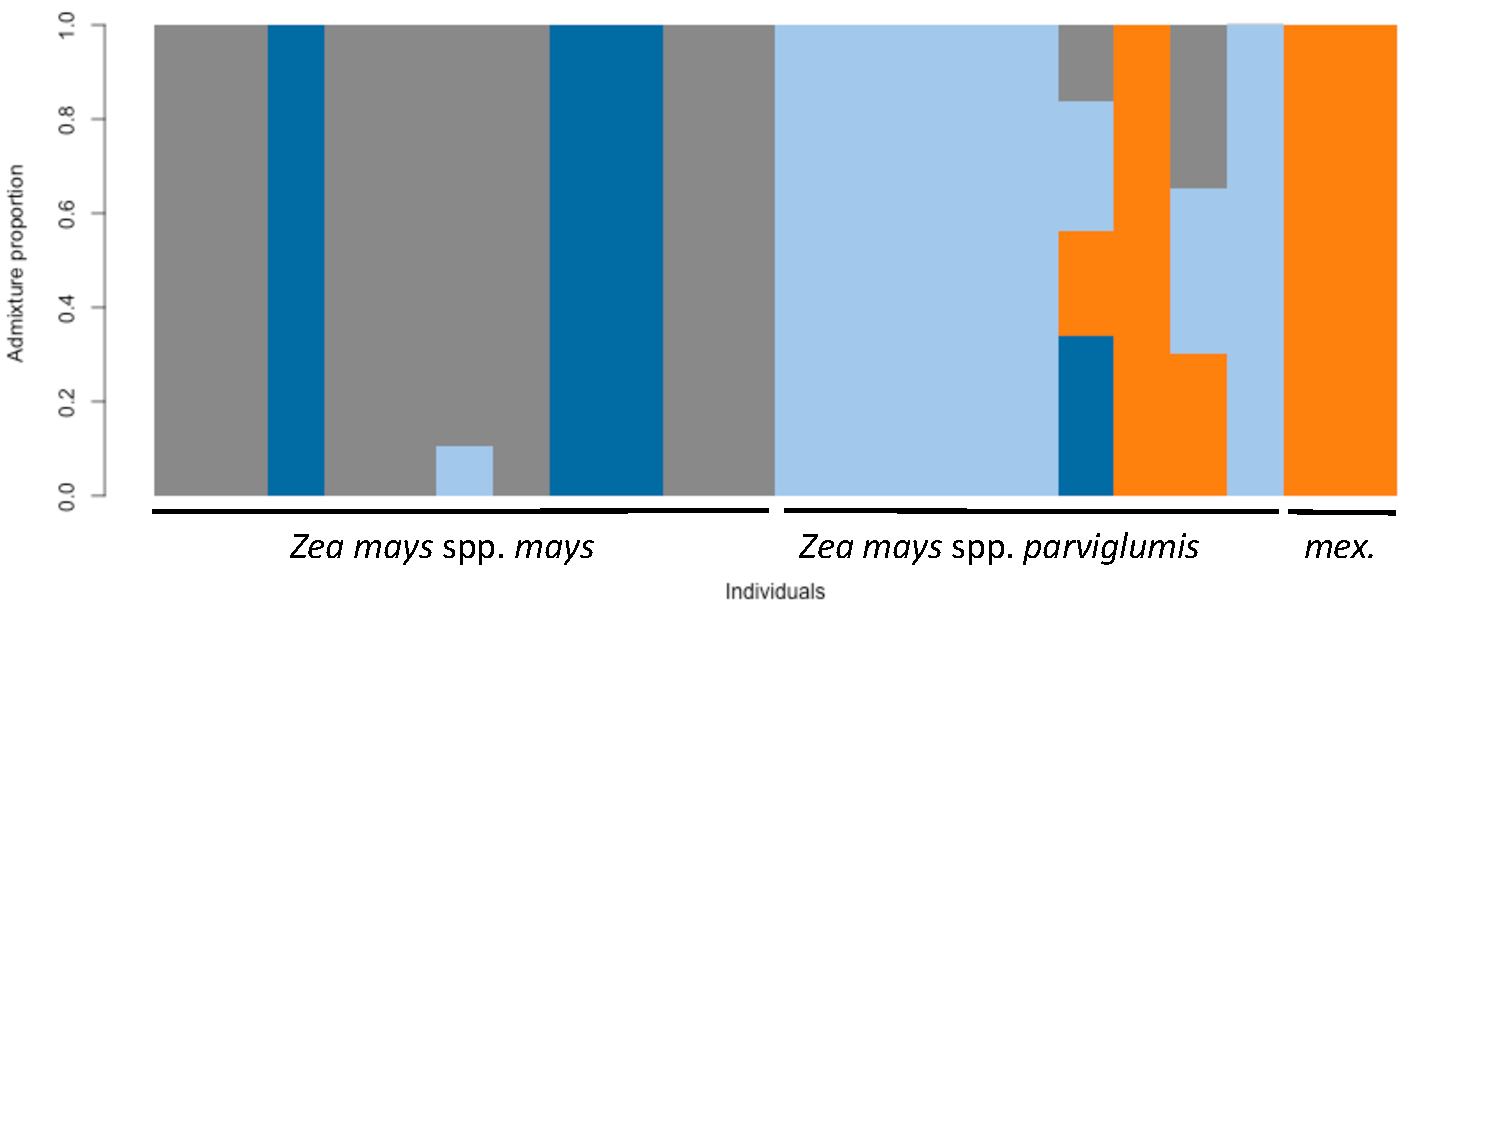
\includegraphics[width=0.8\linewidth]{figures/mt4labeled.pdf}
\caption{Admixture analysis for {\it Zea mays} ssp. {\it mays}, {\it Zea mays} ssp. {\it parviglumis}, and {\it Zea mays} ssp. {\it mexicana} (\textit{mex}) with colors representing the K=4 source populations. 
Individuals are shown in the same order as Table \ref{tab:samples}. }
\label{fig:admixture}
\end{figure}
\jri{what are vertical lines in pi density plot? need to be consistent about saying "nucleotide diversity" vs "pairwise diversity" vs "pairwise differences" etc.  I vote for "pairwise nucleotide diversity"}
Finally, we include two samples of the related wild teosinte \textit{Zea mays} ssp. \textit{mexicana} to assess evidence for admixture.  
Using the ``Admixture'' method, which implements an estimate of admixture proportion from genotype likelihoods \citep{pmid24026093}, we identify structure within domesticated maize separating three high-latitude temperate landraces from the other tropical accessions (Figure \ref{fig:admixture}). 
This analysis is a supervised method that assigns proportions of the each individual's genome to a putative source population, represented by the colors. 
We ran this analysis over a range of number of ancestral populations (K= 2, 3, 4; See Figure \ref{fig:suppadmix}) and chose the value with the maximum likelihood while keeping the number of parameters as low as possible. 
In maize, we see that most individuals come from one source population (dark grey or dark blue), which is evidence for no admixture between these lowland maize samples and  ssp. \textit{mexicana}, and is consistent with an independent analysis from SNP genotyping \citep{hufford2013genomic}.
\textit{Zea mays} ssp. \textit{mexicana} clusters into its own group (orange), along with a single accession of ssp. \textit{parviglumis} collected from a region in which many teosinte populations appear to be the result of admixture between the two subspecies \citep{fang2012megabase}.  
A single ssp. \textit{parviglumis} accession from the Northern extent of the range does not appear to be well-classified with these data, likely due to our relatively limited geographic and genomic sampling.

\section*{Conclusions}
ANGSD-wrapper provides an easy-to-use interface that simplifies many population genetic analyses implemented in ANGSD \citep{korneliussen2014angsd} and permits the exploration of genome-scale results through interactive visualization.
ANGSD-wrapper is under active development to incorporate updates to the ANGSD software package.  
\section*{Acknowledgements}
We acknowledge funding support from the US National Science Foundation (IOS-1238014 to JRI and IOS-1339393 to PLM), from a University of Minnesota Doctoral Dissertation Fellowship supporting TJYK, and from the University of California Davis Plant Sciences Department. We thank members of the Ross-Ibarra and Morrell Labs for discussion and software testing. We thank the authors of ANGSD and related programs for answering questions, particularly Matteo Fumagalli and Filipe Vieira. Finally, we would like to thank Felix Andrews for statistical advice, although we did not follow it. 
\clearpage
\bibliographystyle{apa}
\bibliography{references}

\renewcommand{\thefigure}{S\arabic{figure}}
\renewcommand{\thetable}{S\arabic{table}}
\setcounter{figure}{0}
\setcounter{table}{0}

\begin{figure}
\centering
\caption{Workflow diagram for all methods available in ANGSD-wrapper.}
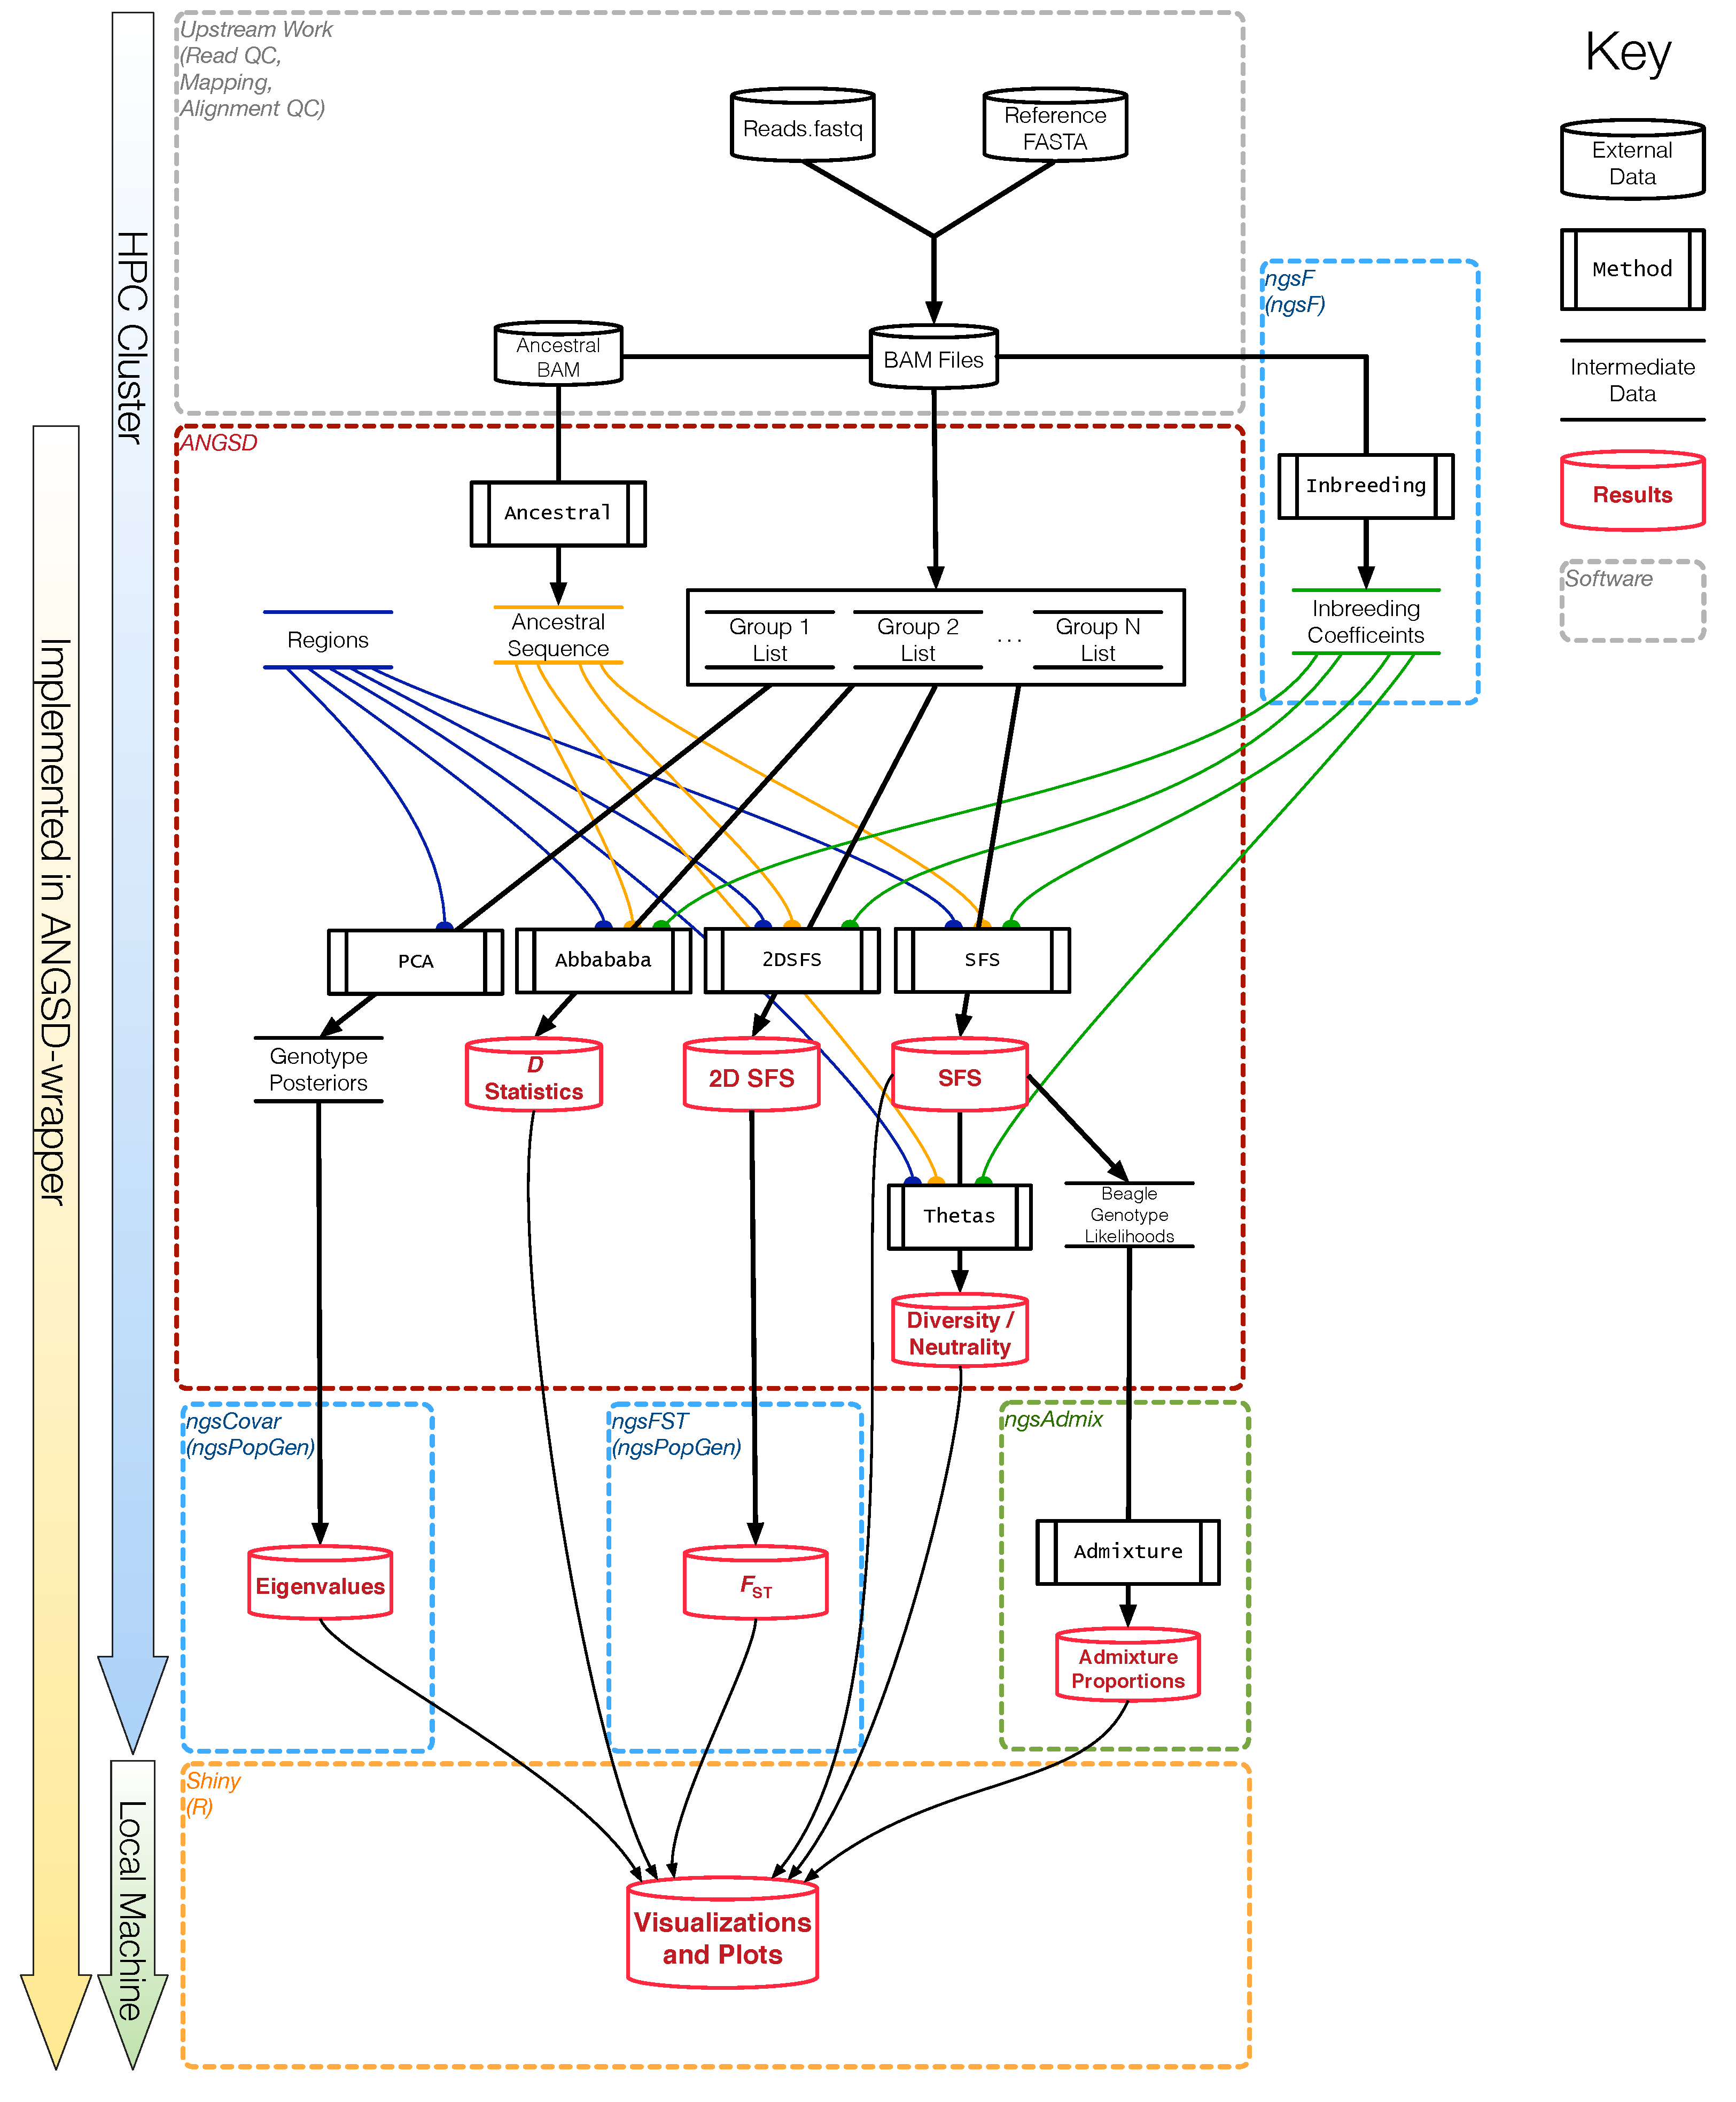
\includegraphics[width=\linewidth]{figures/Big_Workflow_newAW.pdf}
\label{fig:supp2}
\end{figure}

\begin{figure}
\centering
\caption{Admixture analysis for K=2 (top), K=3 (middle), and K=4 (bottom).}
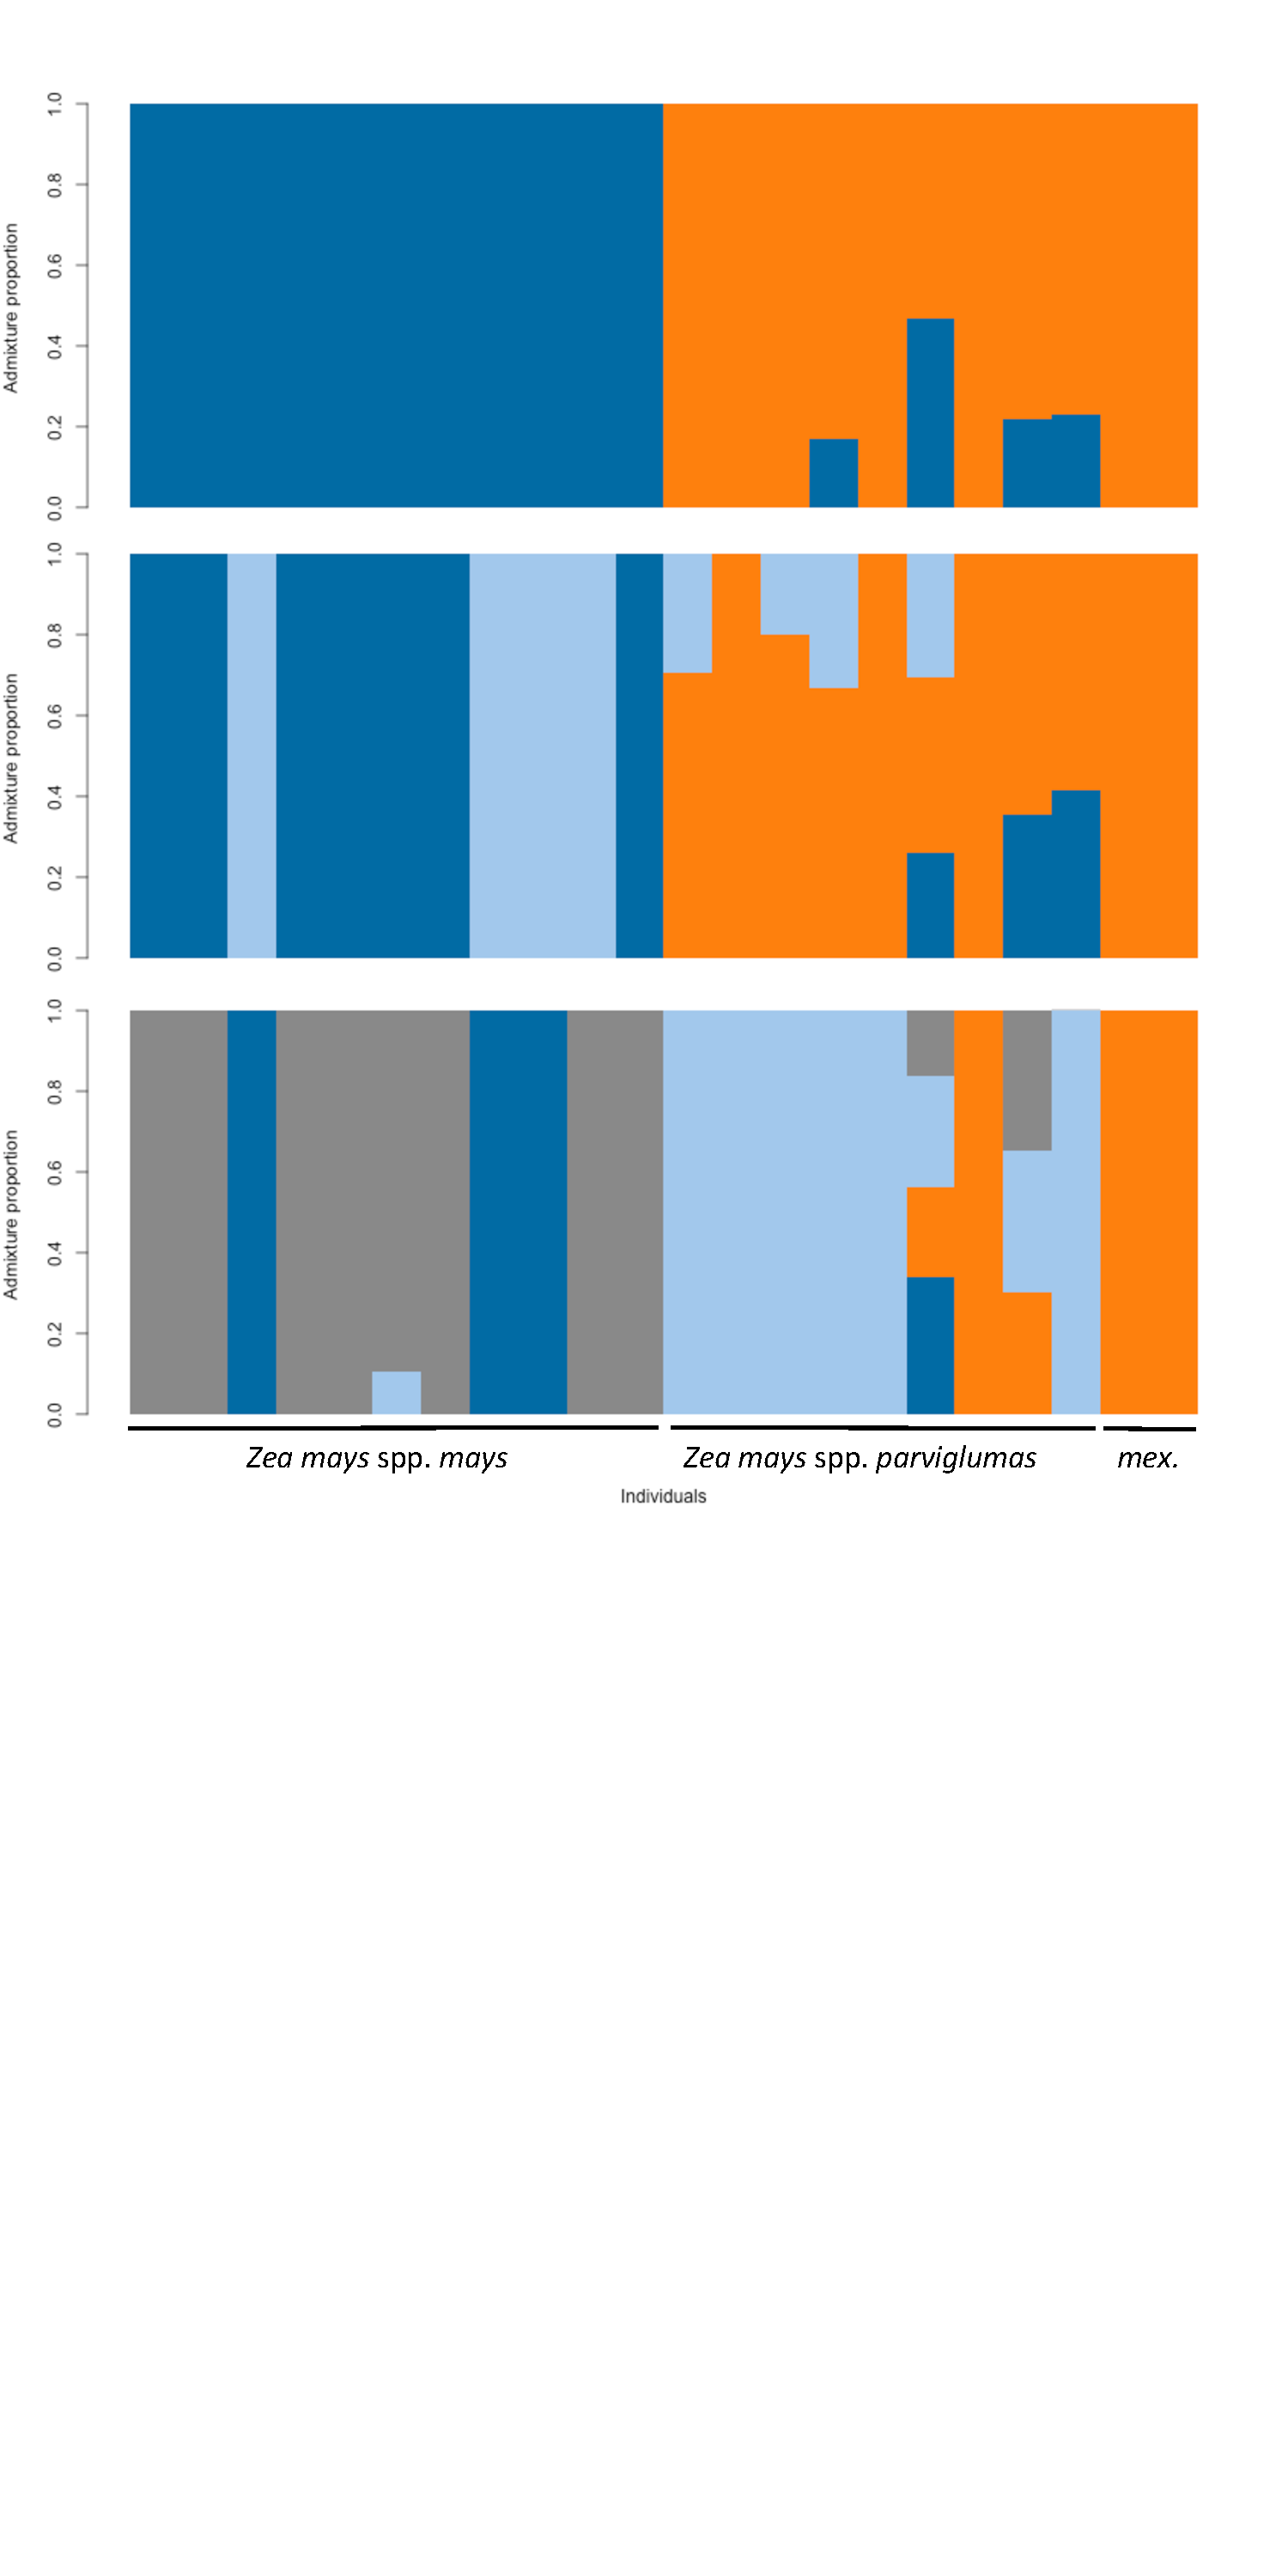
\includegraphics[width=\linewidth]{figures/admixture.pdf}
\label{fig:suppadmix}
\end{figure}

\begin{figure}
\centering
\caption{\fst values plotted against base pair position on chromosome 10 of maize. \fst is calculated between the maize and teosinte samples.}
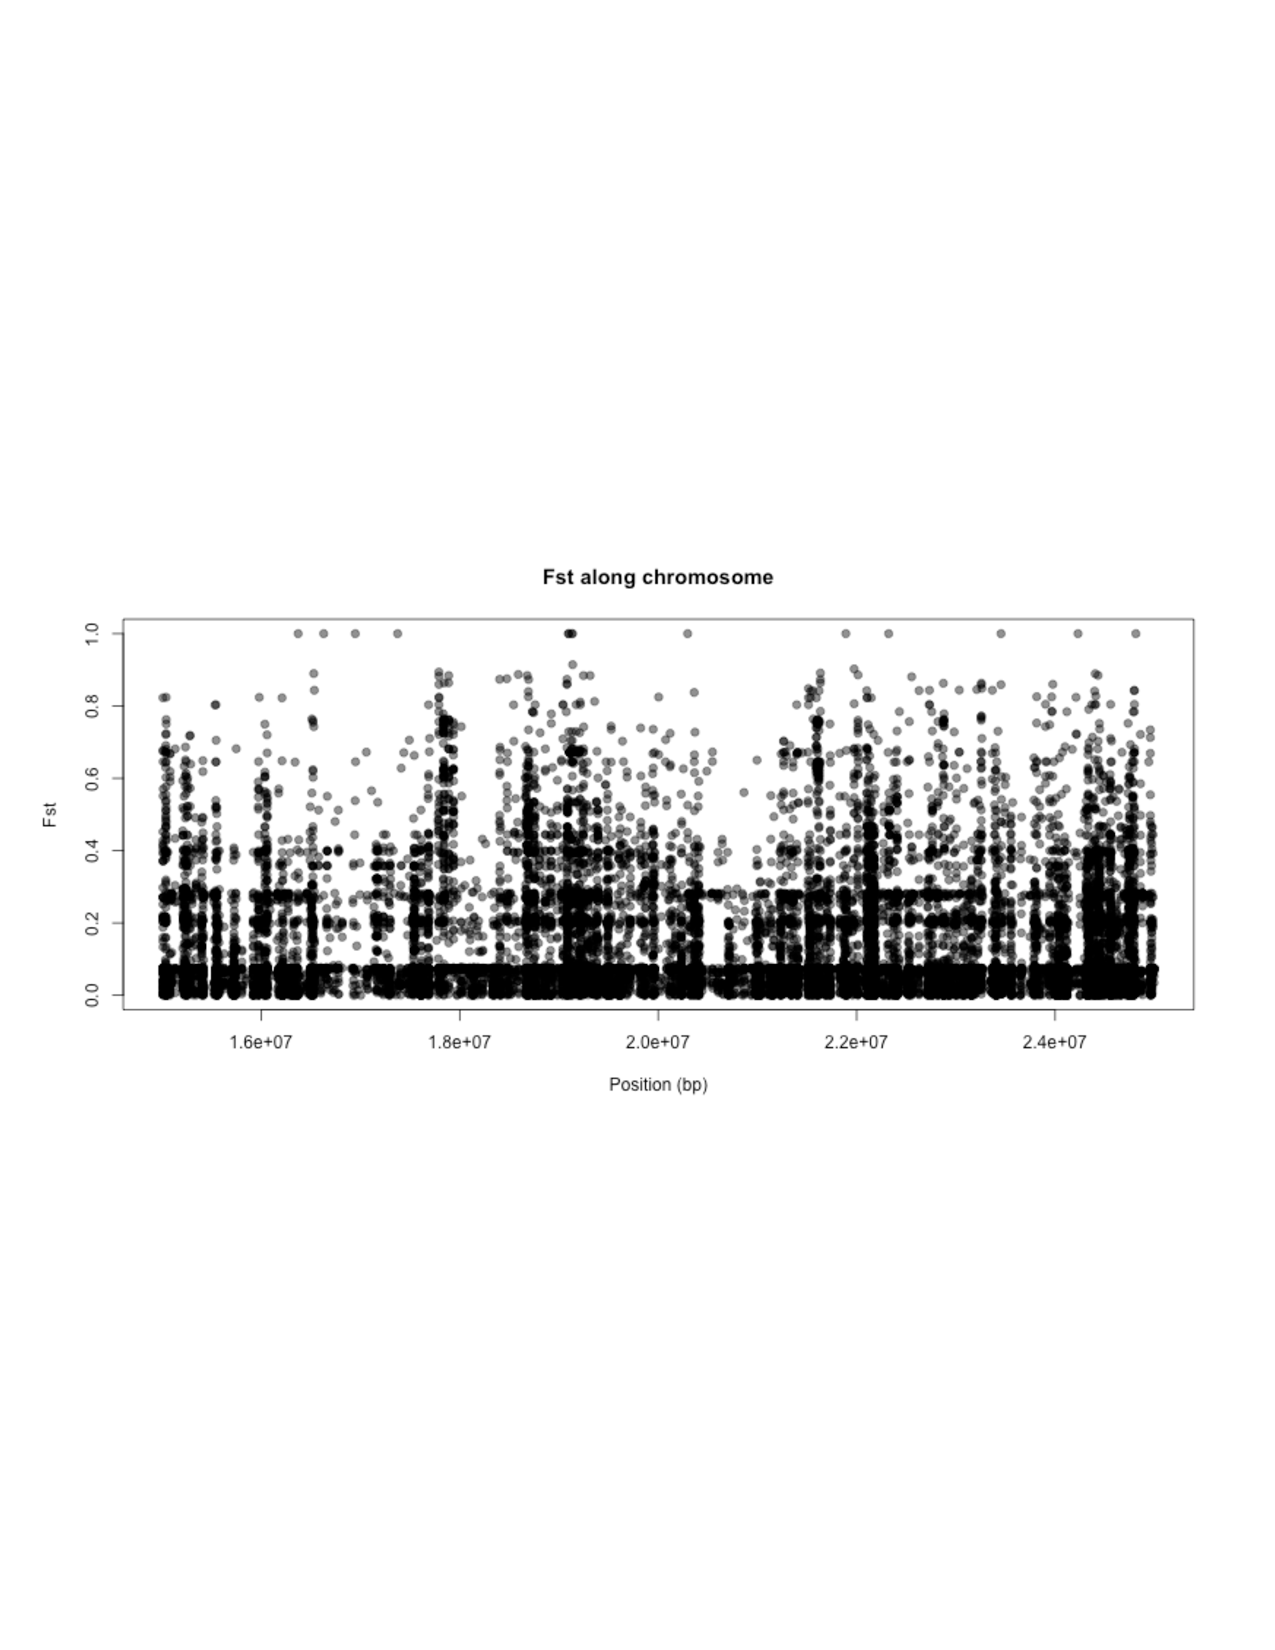
\includegraphics[width=\linewidth]{figures/supp3.pdf}
\label{fig:suppfst}
\end{figure}

\begin{table}
\begin{center}
	\caption{Table of samples used in analysis with mean depth over the region 15000000-25000000 on chromosome 10.}
	\begin{tabular} { | p{5cm} | p{5cm} | p{5cm} | }
	\hline
	\textbf{Sample} & \textbf{Mean Depth} & \textbf{Species} \\ \hline
	BKN009 & 7.00194 & {\it Zea mays} spp. {\it mays}\\ \hline
	BKN011 & 6.9777  & {\it Zea mays} spp. {\it mays}\\ \hline
	BKN014 & 6.78829 & {\it Zea mays} spp. {\it mays} \\ \hline
	BKN015 & 3.739 & {\it Zea mays} spp. {\it mays} \\ \hline
	BKN019 & 3.71944 & {\it Zea mays} spp. {\it mays} \\ \hline
	BKN022 & 3.71268 & {\it Zea mays} spp. {\it mays} \\ \hline
	BKN025 & 3.53799 & {\it Zea mays} spp. {\it mays} \\ \hline
	BKN026 & 3.91798 & {\it Zea mays} spp. {\it mays} \\ \hline
	BKN027 & 7.05576 & {\it Zea mays} spp. {\it mays} \\ \hline
	BKN033 & 3.85336 & {\it Zea mays} spp. {\it mays} \\ \hline
	BKN035 & 3.74839 & {\it Zea mays} spp. {\it mays} \\ \hline
	TIL01 & 3.60133 & {\it Zea mays} spp. {\it parviglumis}\\ \hline
	TIL03 & 4.07518 & {\it Zea mays} spp. {\it parviglumis} \\ \hline
	TIL04 & 6.09163 & {\it Zea mays} spp. {\it parviglumis} \\ \hline
	TIL07 & 5.11419 & {\it Zea mays} spp. {\it parviglumis} \\ \hline
	TIL09 & 5.29004 & {\it Zea mays} spp. {\it parviglumis} \\ \hline
	TIL11 & 3.15477 & {\it Zea mays} spp. {\it parviglumis} \\ \hline
	TIL15 & 6.87873 & {\it Zea mays} spp. {\it parviglumis} \\ \hline
	TIL16 & 2.67186 & {\it Zea mays} spp. {\it parviglumis} \\ \hline
	TIL17 & 2.61892 & {\it Zea mays} spp. {\it parviglumis} \\ \hline
	TIL08 & 6.09453 & \textit{Zea mays} ssp. {\it mexicana} \\ \hline
	TIL25 & 13.1566 & \textit{Zea mays} ssp. {\it mexicana} \\ \hline
	TDD39103 & 8.62 & \textit{Tripsacum dactyloides} \\ \hline
	\end{tabular}
	\label{tab:samples}
	\end{center}
\end{table}


\end{document}
